\documentclass[11pt]{article}
\usepackage[margin=1in]{geometry}
\usepackage{booktabs,amsmath,amssymb,amsthm,graphicx,url,array,xcolor}
\usepackage[colorlinks=true,linkcolor=blue!50!black,citecolor=blue!50!black,urlcolor=blue!50!black]{hyperref}
% AUTO-GENERATED by make_numbers.py. Do not edit.
\newcommand{\OneMismatchShared}{0/900} % H1_H3/*/O1_mismatch_rate_shared
\newcommand{\OneMismatchNaive}{0/900} % H1_H3/*/O1_mismatch_rate_naive
\newcommand{\OneMismatchKeyed}{0/900} % H1_H3/*/O1_mismatch_rate_keyed
\newcommand{\RhoTwoShared}{0.80} % H1_H3/S2/rho/shared
\newcommand{\RhoTwoSharedCI}{[0.66, 0.89]} % H1_H3/S2/rho/shared/ci
\newcommand{\RhoTwoNaive}{0.63} % H1_H3/S2/rho/naive
\newcommand{\RhoTwoNaiveCI}{[0.28, 0.82]} % H1_H3/S2/rho/naive/ci
\newcommand{\RhoTwoKeyed}{0.86} % H1_H3/S2/rho/keyed
\newcommand{\RhoTwoKeyedCI}{[0.65, 0.95]} % H1_H3/S2/rho/keyed/ci
\newcommand{\DeltaRhoTwo}{0.06} % H1_H3/S2/delta_rho_keyed_minus_shared
\newcommand{\DeltaRhoTwoCI}{[-0.16, 0.23]} % H1_H3/S2/delta_rho_keyed_minus_shared/ci
\newcommand{\DeltaRhoNaiveTwo}{0.23} % H1_H3/S2/delta_rho_keyed_minus_naive
\newcommand{\DeltaRhoNaiveTwoCI}{[-0.04, 0.58]} % H1_H3/S2/delta_rho_keyed_minus_naive/ci
\newcommand{\VRFTwo}{1.24} % H1_H3/S2/VRF_shared_over_keyed
\newcommand{\VRFTwoCI}{[0.57, 2.89]} % H1_H3/S2/VRF_shared_over_keyed/ci
\newcommand{\WidthRatioTwo}{0.88} % H1_H3/S2/H3_width_ratio_keyed_over_shared
\newcommand{\HOneVerdictTwo}{not supported} % H1_H3/S2/H1_confirmed
\newcommand{\HThreeVerdictTwo}{not confirmed} % H1_H3/S2/H3_confirmed
\newcommand{\MeanDTwoShared}{-0.040} % H1_H3/S2/H3_mean_d_shared/mean
\newcommand{\MeanDTwoSharedCI}{[-0.064, -0.017]} % H1_H3/S2/H3_mean_d_shared/ci
\newcommand{\PValTwoShared}{0.0008} % H1_H3/S2/H3_mean_d_shared/signflip_p
\newcommand{\MeanDTwoNaive}{-0.015} % H1_H3/S2/H3_mean_d_naive/mean
\newcommand{\MeanDTwoNaiveCI}{[-0.041, 0.010]} % H1_H3/S2/H3_mean_d_naive/ci
\newcommand{\PValTwoNaive}{0.2521} % H1_H3/S2/H3_mean_d_naive/signflip_p
\newcommand{\MeanDTwoKeyed}{-0.008} % H1_H3/S2/H3_mean_d_keyed/mean
\newcommand{\MeanDTwoKeyedCI}{[-0.028, 0.013]} % H1_H3/S2/H3_mean_d_keyed/ci
\newcommand{\PValTwoKeyed}{0.4535} % H1_H3/S2/H3_mean_d_keyed/signflip_p
\newcommand{\PropCDiffTwo}{0.016} % H1_H3/S2/PropC_FIFO_mean_M
\newcommand{\PropCSETwo}{0.028} % H1_H3/S2/PropC_FIFO_mean_M
\newcommand{\PropCOKTwo}{yes} % H1_H3/S2/PropC_FIFO_mean_M
\newcommand{\RhoFourShared}{0.66} % H1_H3/S4/rho/shared
\newcommand{\RhoFourSharedCI}{[0.48, 0.82]} % H1_H3/S4/rho/shared/ci
\newcommand{\RhoFourNaive}{0.75} % H1_H3/S4/rho/naive
\newcommand{\RhoFourNaiveCI}{[0.64, 0.84]} % H1_H3/S4/rho/naive/ci
\newcommand{\RhoFourKeyed}{0.69} % H1_H3/S4/rho/keyed
\newcommand{\RhoFourKeyedCI}{[0.56, 0.80]} % H1_H3/S4/rho/keyed/ci
\newcommand{\DeltaRhoFour}{0.03} % H1_H3/S4/delta_rho_keyed_minus_shared
\newcommand{\DeltaRhoFourCI}{[-0.18, 0.24]} % H1_H3/S4/delta_rho_keyed_minus_shared/ci
\newcommand{\DeltaRhoNaiveFour}{-0.05} % H1_H3/S4/delta_rho_keyed_minus_naive
\newcommand{\DeltaRhoNaiveFourCI}{[-0.22, 0.09]} % H1_H3/S4/delta_rho_keyed_minus_naive/ci
\newcommand{\VRFFour}{0.79} % H1_H3/S4/VRF_shared_over_keyed
\newcommand{\VRFFourCI}{[0.37, 1.58]} % H1_H3/S4/VRF_shared_over_keyed/ci
\newcommand{\WidthRatioFour}{1.14} % H1_H3/S4/H3_width_ratio_keyed_over_shared
\newcommand{\HOneVerdictFour}{not supported} % H1_H3/S4/H1_confirmed
\newcommand{\HThreeVerdictFour}{not confirmed} % H1_H3/S4/H3_confirmed
\newcommand{\MeanDFourShared}{-0.026} % H1_H3/S4/H3_mean_d_shared/mean
\newcommand{\MeanDFourSharedCI}{[-0.051, 0.002]} % H1_H3/S4/H3_mean_d_shared/ci
\newcommand{\PValFourShared}{0.0645} % H1_H3/S4/H3_mean_d_shared/signflip_p
\newcommand{\MeanDFourNaive}{-0.034} % H1_H3/S4/H3_mean_d_naive/mean
\newcommand{\MeanDFourNaiveCI}{[-0.058, -0.010]} % H1_H3/S4/H3_mean_d_naive/ci
\newcommand{\PValFourNaive}{0.0076} % H1_H3/S4/H3_mean_d_naive/signflip_p
\newcommand{\MeanDFourKeyed}{-0.041} % H1_H3/S4/H3_mean_d_keyed/mean
\newcommand{\MeanDFourKeyedCI}{[-0.072, -0.012]} % H1_H3/S4/H3_mean_d_keyed/ci
\newcommand{\PValFourKeyed}{0.0083} % H1_H3/S4/H3_mean_d_keyed/signflip_p
\newcommand{\PropCDiffFour}{0.007} % H1_H3/S4/PropC_FIFO_mean_M
\newcommand{\PropCSEFour}{0.027} % H1_H3/S4/PropC_FIFO_mean_M
\newcommand{\PropCOKFour}{yes} % H1_H3/S4/PropC_FIFO_mean_M
\newcommand{\RhoEightShared}{0.73} % H1_H3/S8/rho/shared
\newcommand{\RhoEightSharedCI}{[0.58, 0.85]} % H1_H3/S8/rho/shared/ci
\newcommand{\RhoEightNaive}{0.65} % H1_H3/S8/rho/naive
\newcommand{\RhoEightNaiveCI}{[0.49, 0.79]} % H1_H3/S8/rho/naive/ci
\newcommand{\RhoEightKeyed}{0.86} % H1_H3/S8/rho/keyed
\newcommand{\RhoEightKeyedCI}{[0.76, 0.92]} % H1_H3/S8/rho/keyed/ci
\newcommand{\DeltaRhoEight}{0.13} % H1_H3/S8/delta_rho_keyed_minus_shared
\newcommand{\DeltaRhoEightCI}{[-0.02, 0.30]} % H1_H3/S8/delta_rho_keyed_minus_shared/ci
\newcommand{\DeltaRhoNaiveEight}{0.21} % H1_H3/S8/delta_rho_keyed_minus_naive
\newcommand{\DeltaRhoNaiveEightCI}{[0.05, 0.37]} % H1_H3/S8/delta_rho_keyed_minus_naive/ci
\newcommand{\VRFEight}{1.37} % H1_H3/S8/VRF_shared_over_keyed
\newcommand{\VRFEightCI}{[0.75, 2.58]} % H1_H3/S8/VRF_shared_over_keyed/ci
\newcommand{\WidthRatioEight}{0.85} % H1_H3/S8/H3_width_ratio_keyed_over_shared
\newcommand{\HOneVerdictEight}{not supported} % H1_H3/S8/H1_confirmed
\newcommand{\HThreeVerdictEight}{not confirmed} % H1_H3/S8/H3_confirmed
\newcommand{\MeanDEightShared}{-0.026} % H1_H3/S8/H3_mean_d_shared/mean
\newcommand{\MeanDEightSharedCI}{[-0.058, 0.005]} % H1_H3/S8/H3_mean_d_shared/ci
\newcommand{\PValEightShared}{0.1128} % H1_H3/S8/H3_mean_d_shared/signflip_p
\newcommand{\MeanDEightNaive}{-0.035} % H1_H3/S8/H3_mean_d_naive/mean
\newcommand{\MeanDEightNaiveCI}{[-0.065, -0.004]} % H1_H3/S8/H3_mean_d_naive/ci
\newcommand{\PValEightNaive}{0.0290} % H1_H3/S8/H3_mean_d_naive/signflip_p
\newcommand{\MeanDEightKeyed}{-0.033} % H1_H3/S8/H3_mean_d_keyed/mean
\newcommand{\MeanDEightKeyedCI}{[-0.060, -0.006]} % H1_H3/S8/H3_mean_d_keyed/ci
\newcommand{\PValEightKeyed}{0.0177} % H1_H3/S8/H3_mean_d_keyed/signflip_p
\newcommand{\PropCDiffEight}{0.018} % H1_H3/S8/PropC_FIFO_mean_M
\newcommand{\PropCSEEight}{0.033} % H1_H3/S8/PropC_FIFO_mean_M
\newcommand{\PropCOKEight}{yes} % H1_H3/S8/PropC_FIFO_mean_M
\newcommand{\CostShared}{3.13} % H1_H3/S2/cost_wall_ms/shared/median_ms
\newcommand{\CostNaive}{4.18} % H1_H3/S2/cost_wall_ms/naive/median_ms
\newcommand{\CostKeyed}{7.44} % H1_H3/S2/cost_wall_ms/keyed/median_ms
\newcommand{\CostRatioKeyed}{2.38} % H1_H3/S2/cost_wall_ms keyed/shared
\newcommand{\UndelFracFIFO}{1.2\%} % H2/S2/FIFO/undelivered_fraction
\newcommand{\UndelFracFIFOCI}{[1.0\%, 1.3\%]} % H2/S2/FIFO/undelivered_fraction/ci
\newcommand{\UnderUFIFO}{-0.4\%} % H2/S2/FIFO/understatement_U
\newcommand{\UnderUFIFOCI}{[-0.5\%, -0.3\%]} % H2/S2/FIFO/understatement_U/ci
\newcommand{\UndelFracFullSASP}{1.2\%} % H2/S2/FullSASP/undelivered_fraction
\newcommand{\UndelFracFullSASPCI}{[1.0\%, 1.4\%]} % H2/S2/FullSASP/undelivered_fraction/ci
\newcommand{\UnderUFullSASP}{-0.2\%} % H2/S2/FullSASP/understatement_U
\newcommand{\UnderUFullSASPCI}{[-0.4\%, -0.1\%]} % H2/S2/FullSASP/understatement_U/ci
\newcommand{\UndelFracMeanOnly}{1.2\%} % H2/S2/MeanOnly/undelivered_fraction
\newcommand{\UndelFracMeanOnlyCI}{[1.0\%, 1.4\%]} % H2/S2/MeanOnly/undelivered_fraction/ci
\newcommand{\UnderUMeanOnly}{-0.3\%} % H2/S2/MeanOnly/understatement_U
\newcommand{\UnderUMeanOnlyCI}{[-0.4\%, -0.1\%]} % H2/S2/MeanOnly/understatement_U/ci
\newcommand{\LateDiscards}{0.00} % H2/S2/*/late_discards_per_run (max)
\newcommand{\RetryDrops}{0.00} % H2/S2/*/dropped_after_retry_per_run (max)
\newcommand{\GenPerRun}{238} % H2/S2/FIFO/generated_per_run
\newcommand{\DrainValid}{passed} % H2/drain_control/validity_check_passed
\newcommand{\DrainRows}{300} % H2/drain_control/fer0_rows
\newcommand{\DrainUndelFerOne}{0.00} % H2/drain_control/fer001_undelivered_per_run (max)
\newcommand{\RankFlip}{6\%} % H2/exploratory_ranking_flip_fraction_S2
\newcommand{\UndelThreshold}{2\%} % preregistration H2 threshold (constant)
\newcommand{\HTwoVerdict}{not material} % H2/*/all_arms_material
\newcommand{\HFourRatioFIFO}{54\%} % H4/FIFO/ratio
\newcommand{\HFourRatioFIFOCI}{[37\%, 75\%]} % H4/FIFO/ratio_ci
\newcommand{\HFourWithFIFO}{0.0049} % H4/FIFO/mean_S1_with
\newcommand{\HFourWithoutFIFO}{0.0057} % H4/FIFO/mean_S1_without
\newcommand{\HFourAbsFIFO}{0.0027} % H4/FIFO/mean_abs_diff
\newcommand{\HFourRatioFullSASP}{53\%} % H4/FullSASP/ratio
\newcommand{\HFourRatioFullSASPCI}{[38\%, 72\%]} % H4/FullSASP/ratio_ci
\newcommand{\HFourWithFullSASP}{0.0060} % H4/FullSASP/mean_S1_with
\newcommand{\HFourWithoutFullSASP}{0.0057} % H4/FullSASP/mean_S1_without
\newcommand{\HFourAbsFullSASP}{0.0031} % H4/FullSASP/mean_abs_diff
\newcommand{\HFourTrace}{0.0} % H4/FIFO/trace_control_max_abs_diff
\newcommand{\HFourVerdict}{confirmed} % H4/FIFO/violation_confirmed
\newcommand{\HFourUnits}{2.7} % H4/FIFO/mean_abs_diff x 1000 (microseconds)
\newcommand{\OFiveRate}{100\%} % H5/O5_shipped/violation_rate
\newcommand{\OFiveAttempts}{23{,}963} % H5/O5_shipped/attempts
\newcommand{\OFiveSingleRate}{0\%} % H5/O5_single/violation_rate
\newcommand{\BurstShipped}{1.25} % H5/burst_run_length/shipped
\newcommand{\BurstSingle}{1.76} % H5/burst_run_length/single
\newcommand{\BurstRel}{-29\%} % H5/burst_run_length/rel_diff
\newcommand{\BurstRelAbs}{29\%} % H5/burst_run_length/rel_diff (absolute value)
\newcommand{\BurstRelCI}{[-34\%, -24\%]} % H5/burst_run_length/ci
\newcommand{\HFiveVerdict}{confirmed} % H5/burst_run_length/material
\newcommand{\LossFreqShipped}{0.0098} % H5/loss_frequency_nobursts_shipped/freq
\newcommand{\LossFreqShippedCI}{[0.0086, 0.0111]} % H5/loss_frequency_nobursts_shipped/exact95
\newcommand{\LossFreqSingle}{0.0101} % H5/loss_frequency_nobursts_single/freq
\newcommand{\LossFreqSingleCI}{[0.0089, 0.0115]} % H5/loss_frequency_nobursts_single/exact95
\newcommand{\HSixFIFO}{0/100} % H6/FIFO
\newcommand{\HSixFullSASP}{0/100} % H6/FullSASP
\newcommand{\HSixMeanOnly}{0/100} % H6/MeanOnly
\newcommand{\HSixLeakyGlobal}{100/100} % H6/LeakyGlobal
\newcommand{\HSixLeakyLocal}{0/100} % H6/LeakyLocal
\newcommand{\HSixVerdict}{pass} % H6/pass
\newcommand{\EOneTotal}{0/500} % E1 (sum)
\newcommand{\XOneMismatch}{0} % X1 (sum of arrival mismatches)
\newcommand{\XOneRhoLow}{0.67} % X1/delta_mu_0.1/shared/rho
\newcommand{\XOneRhoHigh}{-0.06} % X1/delta_mu_2.0/shared/rho
\newcommand{\XOneRhoHighKeyed}{0.03} % X1/delta_mu_2.0/keyed/rho
\newcommand{\XTwoMShipFIFO}{0.83} % X2/shipped_FIFO/M_mean
\newcommand{\XTwoMSingleFIFO}{1.91} % X2/single_FIFO/M_mean
\newcommand{\XTwoMShipSASP}{0.57} % X2/shipped_FullSASP/M_mean
\newcommand{\XTwoMSingleSASP}{1.34} % X2/single_FullSASP/M_mean
\newcommand{\XTwoRedShip}{32\%} % X2 relative reduction shipped
\newcommand{\XTwoRedSingle}{30\%} % X2 relative reduction single
\newcommand{\XTwoUndelShip}{1.2\%} % X2/shipped_FIFO/undelivered_frac
\newcommand{\XTwoUndelSingle}{3.1\%} % X2/single_FIFO/undelivered_frac
\newcommand{\XThreeFIFO}{0/100} % X3/FIFO
\newcommand{\XThreeFullSASP}{0/100} % X3/FullSASP
\newcommand{\XThreeMeanOnly}{0/100} % X3/MeanOnly
\newcommand{\XThreeLeakyGlobal}{94/100} % X3/LeakyGlobal
\newcommand{\XThreeLeakyLocal}{20/100} % X3/LeakyLocal
\newcommand{\XFourDKeyed}{-0.014} % X4/keyed/mean_d
\newcommand{\XFourCIKeyed}{[-0.022, -0.007]} % X4/keyed/ci
\newcommand{\XFourFIFOKeyed}{0.119} % X4/keyed/mean_FIFO
\newcommand{\XFourSASPKeyed}{0.105} % X4/keyed/mean_FullSASP
\newcommand{\XFourLowerKeyed}{56\%} % X4/keyed/frac_seeds_sasp_lower
\newcommand{\XFourDShared}{-0.018} % X4/shared/mean_d
\newcommand{\XFourCIShared}{[-0.026, -0.009]} % X4/shared/ci
\newcommand{\XFourFIFOShared}{0.119} % X4/shared/mean_FIFO
\newcommand{\XFourSASPShared}{0.101} % X4/shared/mean_FullSASP
\newcommand{\XFourLowerShared}{56\%} % X4/shared/frac_seeds_sasp_lower
\newcommand{\XFourRel}{12\%} % X4 relative reduction (keyed)
\newcommand{\XFiveIdentical}{100\%} % X5/traffic_identical_fraction
\newcommand{\XFiveTriples}{270} % X5/n_triples
\newcommand{\XFiveRhoMin}{-0.32} % X5 min rho over cells
\newcommand{\XFiveRhoMax}{0.98} % X5 max rho over cells
\newcommand{\OldFIFO}{0.159} % experiments/ablation_phase6/raw_runs.csv RegimeA w50 DefaultFIFO mean weighted_cost
\newcommand{\OldSASP}{0.099} % same, FullSASP
\newcommand{\OldRel}{38\%} % same, relative reduction
\newcommand{\OldN}{30} % same, runs per arm
\newcommand{\OldD}{-0.060} % same, mean paired difference FullSASP-FIFO per seed
\newcommand{\OldDCI}{[-0.115, -0.008]} % same, seed-bootstrap 95% CI (10000, default_rng(20261017))
\newcommand{\OldRatio}{3.4} % OldD / X4 shared mean_d
\newcommand{\SBrFour}{0.7\%} % S4/FIFO/explained_fraction
\newcommand{\SBrFourCI}{[0.6\%, 0.8\%]} % S4/FIFO/explained_fraction/ci
\newcommand{\SBtauFour}{0.18} % S4/FIFO/kendall_trace_vs_shapley/mean
\newcommand{\SBtauFourCI}{[0.10, 0.27]} % S4/FIFO/kendall_trace_vs_shapley/ci
\newcommand{\SBtopFour}{39\%} % S4/FIFO/top_offender_agreement
\newcommand{\SBchanceFour}{25.0\%} % 1/4 (chance agreement)
\newcommand{\SBRFour}{1.90} % S4/FIFO/nonadditivity_R
\newcommand{\SBRFourCI}{[1.86, 1.95]} % S4/FIFO/nonadditivity_R/ci
\newcommand{\SBEFour}{1.10} % S4/FIFO/mean_E_ms
\newcommand{\SBXFour}{0.008} % S4/FIFO/mean_X_ms
\newcommand{\SBVerdictRFour}{confirmed (X does not capture externality)} % S4/FIFO/H7_verdict
\newcommand{\SBVerdictTFour}{confirmed (misranking)} % S4/FIFO/H8_verdict
\newcommand{\SBVerdictNFour}{confirmed (non-additive)} % S4/FIFO/H9_verdict
\newcommand{\SBrEight}{0.7\%} % S8/FIFO/explained_fraction
\newcommand{\SBrEightCI}{[0.6\%, 0.8\%]} % S8/FIFO/explained_fraction/ci
\newcommand{\SBtauEight}{0.16} % S8/FIFO/kendall_trace_vs_shapley/mean
\newcommand{\SBtauEightCI}{[0.10, 0.22]} % S8/FIFO/kendall_trace_vs_shapley/ci
\newcommand{\SBtopEight}{26\%} % S8/FIFO/top_offender_agreement
\newcommand{\SBchanceEight}{12.5\%} % 1/8 (chance agreement)
\newcommand{\SBREight}{2.69} % S8/FIFO/nonadditivity_R
\newcommand{\SBREightCI}{[2.60, 2.78]} % S8/FIFO/nonadditivity_R/ci
\newcommand{\SBEEight}{1.16} % S8/FIFO/mean_E_ms
\newcommand{\SBXEight}{0.008} % S8/FIFO/mean_X_ms
\newcommand{\SBVerdictREight}{confirmed (X does not capture externality)} % S8/FIFO/H7_verdict
\newcommand{\SBVerdictTEight}{confirmed (misranking)} % S8/FIFO/H8_verdict
\newcommand{\SBVerdictNEight}{confirmed (non-additive)} % S8/FIFO/H9_verdict
\newcommand{\SBVone}{0.0} % S4/FIFO/validity/V1
\newcommand{\SBVtwo}{0} % S4/FIFO/validity/V2
\newcommand{\SBVfour}{0.0} % S4/FIFO/validity/V4
\newcommand{\SBVthree}{0.10} % V3_lowload_control/explained_fraction
\newcommand{\SBVthreeStatus}{FAILED} % V3_lowload_control/passed
\newcommand{\SBLowE}{0.39} % LowLoad/FIFO/mean_E_ms
\newcommand{\SBLowX}{0.039} % LowLoad/FIFO/mean_X_ms
\newcommand{\SBNegE}{0.5\%} % max frac_negative_externality over configs
\newcommand{\SBSaspBlameA}{1.06} % S4/FullSASP/mean_blame_SH_by_flow[0]
\newcommand{\SBFifoBlameA}{1.11} % S4/FIFO/mean_blame_SH_by_flow[0]
\newcommand{\SBSaspBlameB}{0.74} % S4/FullSASP/mean_blame_SH_by_flow[1]
\newcommand{\SBFifoBlameB}{1.08} % S4/FIFO/mean_blame_SH_by_flow[1]
\newcommand{\SBSaspBlameC}{1.32} % S4/FullSASP/mean_blame_SH_by_flow[2]
\newcommand{\SBFifoBlameC}{1.10} % S4/FIFO/mean_blame_SH_by_flow[2]
\newcommand{\SBSaspBlameD}{1.27} % S4/FullSASP/mean_blame_SH_by_flow[3]
\newcommand{\SBFifoBlameD}{1.11} % S4/FIFO/mean_blame_SH_by_flow[3]
\newcommand{\SBSaspTau}{0.10} % S4/FullSASP/kendall_trace_vs_shapley/mean
\newcommand{\SBBCrossMin}{0.6\%} % 2b share_cross min (load1.0_asym0.1)
\newcommand{\SBBCrossMax}{36.6\%} % 2b share_cross max (load0.5_asym5.0)
\newcommand{\SBBCrossMed}{8.0\%} % 2b share_cross median over 12 cells
\newcommand{\SBBCrossBelowFifteen}{10/12} % 2b cells with share_cross < 15%
\newcommand{\SBBNetMin}{60\%} % 2b share_net min
\newcommand{\SBBNetMax}{99\%} % 2b share_net max
\newcommand{\SBBSelfAbs}{4.9\%} % 2b max |share_self|
\newcommand{\SBBIdentity}{1.4e-14} % 2b checks V5
\newcommand{\SBBSolo}{0.0} % 2b checks V6
\newcommand{\SBBCells}{12} % 2b number of cells
\newcommand{\SBBMaxCrossLoad}{0.5} % 2b load at max share (load0.5_asym5.0)
\newcommand{\SBBMaxCrossAsym}{5.0} % 2b asymmetry at max share (load0.5_asym5.0)
\newcommand{\SBBMinCrossLoad}{1.0} % 2b load at min share (load1.0_asym0.1)
\newcommand{\TenGapPinned}{0.1\%} % S3py H10/P256/gap/point
\newcommand{\TenGapPinnedCI}{[0.0\%, 0.4\%]} % S3py H10/P256/gap/ci
\newcommand{\TenGapShared}{99.5\%} % S3py H10/F64/gap/point
\newcommand{\TenGapSharedCI}{[99.3\%, 99.6\%]} % S3py H10/F64/gap/ci
\newcommand{\TenVSeven}{0.0026} % S3py H10/P256/V7_max_abs_E_minus_X_clean_runs
\newcommand{\TenEPinned}{0.0099} % S3py H10/P256/mean_E_ms
\newcommand{\TenESharedF}{0.935} % S3py H10/F64/mean_E_ms
\newcommand{\TwelveFlawSASPDiff}{6.09} % S3py H12/FullSASP/SH_minus_TR/mean
\newcommand{\TwelveFlawSASPCI}{[3.20, 9.16]} % S3py H12/FullSASP/SH_minus_TR/ci
\newcommand{\TwelveFlawTRvsRand}{-8.92} % S3py H12/FullSASP/TR_minus_RAND/mean
\newcommand{\ElevenMin}{4\%} % S3ns3 cells r min
\newcommand{\ElevenMax}{88\%} % S3ns3 cells r max
\newcommand{\ElevenDefined}{9} % S3ns3 n_defined
\newcommand{\ElevenMostly}{4} % S3ns3 n_mostly_explained
\newcommand{\ElevenLittle}{5} % S3ns3 n_little_explained
\newcommand{\ElevenRuns}{270} % S3ns3 n_nobulk_runs
\newcommand{\SXSixMaxStall}{3\%} % S3x X6 max frac_runs_with_stall
\newcommand{\SXSixGapLow}{0.6\%} % S3x X6 load1.0_win64 gap
\newcommand{\SXSixGapHigh}{15.6\%} % S3x X6 load1.4_win64 gap
\newcommand{\SXSixEHigh}{0.011} % S3x X6 load1.4_win64 mean_E_ms
\newcommand{\SXSixGapHighCI}{[0.0\%, 64.6\%]} % S3x X6 load1.4_win64 gap ci
\newcommand{\SXSevenFifoDiff}{-0.088} % S3x X7 FIFO unweighted SH_minus_TR mean
\newcommand{\SXSevenFifoCI}{[-0.194, 0.016]} % S3x X7 FIFO unweighted SH_minus_TR ci
\newcommand{\SXSevenSaspDiff}{0.000} % S3x X7 FullSASP unweighted SH_minus_TR mean
\newcommand{\FourCells}{19} % S4 n_cells
\newcommand{\FourDefined}{19} % S4 n_defined
\newcommand{\FourPyViol}{0/13} % S4 H13 python_violations/python_defined
\newcommand{\FourPyFloorViol}{0/13} % S4 H13 python_floor_violations
\newcommand{\FourNsViol}{0/6} % S4 H13 ns3_violations/ns3_defined
\newcommand{\FourRho}{0.93} % S4 H14 pooled rho
\newcommand{\FourRhoCI}{[0.78, 0.98]} % S4 H14 pooled ci
\newcommand{\FourRhoPy}{0.85} % S4 H14 python rho
\newcommand{\FourRhoNs}{0.60} % S4 H14 ns3 rho
\newcommand{\FourPyQMin}{0.03\%} % S4 python q min
\newcommand{\FourPyQMax}{9.4\%} % S4 python q max
\newcommand{\FourPyRMin}{0.8\%} % S4 python r min
\newcommand{\FourPyRMax}{23.0\%} % S4 python r max
\newcommand{\FourNsQMin}{8\%} % S4 ns3 q min
\newcommand{\FourNsQMax}{35\%} % S4 ns3 q max
\newcommand{\FourNsRMin}{12\%} % S4 ns3 r min
\newcommand{\FourNsRMax}{127\%} % S4 ns3 r max
\newcommand{\FourNsRAboveOne}{2} % S4 ns3 cells with r > 1
\newcommand{\FourRatioMedPy}{3.8} % S4 python median r/q
\newcommand{\FourRatioMaxPy}{26} % S4 python max r/q
\newcommand{\FourRatioMedNs}{2.4} % S4 ns3 median r/q
\newcommand{\FourNsEOverMin}{0.009} % S4 ns3 E of cells with r>1 (min)
\newcommand{\FourNsEOverMax}{0.056} % S4 ns3 E of cells with r>1 (max)
\newcommand{\FourTP}{2} % S4 H15 tp
\newcommand{\FourFP}{0} % S4 H15 fp
\newcommand{\FourFN}{2} % S4 H15 fn
\newcommand{\FourPrec}{1.00} % S4 H15 precision
\newcommand{\FourRecall}{0.50} % S4 H15 recall
\newcommand{\FourOLSSlope}{2.55} % S4 exploratory OLS slope
\newcommand{\FourOLSRsq}{0.57} % S4 exploratory OLS r2
\newcommand{\FourVTenGap}{7.1e-15} % S4 V10 identity_max_gap_all_rows
\newcommand{\FourVTenSig}{0} % S4 V10 replay_signature_violations
\newcommand{\FourVTenRows}{6800} % S4 V10 n_rows
\newcommand{\FourNsRuns}{360} % S4 V11 total ns3 runs

\newcommand{\tagC}{\textsc{conf}}
\newcommand{\tagE}{\textsc{expl}}
\newcommand{\tagP}{\textsc{pre-existing}}
\newcommand{\tagA}{\textsc{analytic}}
\newtheorem{proposition}{Proposition}

\title{Who Blocks Whom? Interventional Externality Accounting\\for Cross-Flow Reordering Delay in Multi-Link Wi-Fi Simulation}
\author{[Authors to be completed by the submitting authors]}
\date{}

\begin{document}
\maketitle

\begin{abstract}
Multi-link Wi-Fi~7 devices resequence the packets of several flows in one Block-Ack reorder buffer, so a slow link can delay packets of unrelated flows.
Studies quantify this \emph{cross-blocking} from receiver traces, which holds the transmission schedule fixed.
We argue that the quantity a scheduler designer or operator needs is the \emph{interventional externality}: how much worse a flow's delay is because another flow exists.
We define it by exact counterfactual replay (identical arrivals and per-packet channel noise, one flow removed), prove an accounting identity that splits it into queueing/service, self-reordering and cross-reordering parts, and attribute it across flows with the Shapley value, whose efficiency holds by construction.
In a preregistered study (100 seeds, four and eight flows), trace-level cross-blocking explained only \SBrFour{} (\SBrFourCI) of the externality at a heavy-load operating point, ranked the offending flows with Kendall's $\tau=\SBtauFour$ (\SBtauFourCI) against Shapley blame, and externalities were strongly non-additive ($R=\SBRFour$).
A preregistered low-load validity control \emph{failed} (explained fraction \SBVthree{}, required 0.75--1.25) because queueing externality never vanishes; we report this and replace the control by an exact-identity sweep (exploratory), in which cross-blocking's share ranges from \SBBCrossMin{} to \SBBCrossMax{} and stays below 15\% in \SBBCrossBelowFifteen{} cells.
A companion preregistered audit of the simulator found that the shared random stream did not break seed pairing, that every attempt draws two loss variables instead of one, and that the earlier 30-seed gain estimate of the studied scheduler was \OldRatio{}$\times$ the 1000-seed estimate.
The evidence comes from one simulator; we state what it does and does not support.
\end{abstract}

\section{Introduction}
When several flows share a reorder buffer, packets of one flow can wait for earlier-numbered packets of another that are still in flight on a slower link.
Wi-Fi~7 multi-link operation (MLO)~\cite{ieee80211be2024} makes this concrete: Block-Ack state and the sequence-number space are shared across links, and links differ in delay and load.
The MLO literature we found concentrates on traffic allocation across links, contention anomalies and analytical delay models~\cite{lopezraventos2022mlo,carrascosa2023understanding}; multipath-TCP schedulers target blocking \emph{within} a flow.
We found no work that asks which \emph{other flows} are responsible for a flow's reordering delay, or how large that responsibility is compared with ordinary queueing.

The standard decomposition (used in the audited codebase and, in the literature we found, implicitly elsewhere) computes cross-blocking from a trace: the extra wait of a packet after all earlier packets of its own flow have arrived.
That is a counterfactual only about the \emph{receiver}: it keeps every transmission time as observed.
The decision-relevant counterfactual is different: remove the other flow and let the system run again.
The two coincide only under conditions we make explicit (Proposition~\ref{prop:cond}); in a work-conserving shared-link system they need not.
Our own simulator audit supplied the first hint: a flow's self-blocking was exactly invariant when its competitor's records were deleted from a trace, but changed by \HFourRatioFIFO{} when the competitor was removed from the system (Section~\ref{sec:audit}).

\paragraph{Contributions, ranked by strength of evidence.}
\begin{enumerate}
  \item \textbf{Concept and exact accounting.} The interventional externality of one flow on another, an identity decomposing it into queueing/service, self-reordering and cross-reordering parts, and Shapley attribution over flows. Machinery checks are exact: Shapley efficiency gap \SBVone{}, replay-signature violations \SBVtwo{}, attribution-completeness gap \SBVfour{} (\tagC{}); identity gap \SBBIdentity{} and a solo-flow control equal to \SBBSolo{} (\tagE{}).
  \item \textbf{Trace-level cross-blocking is a small part of the externality here.} \SBrFour{} at the heavy-load operating point (\tagC{}, with the validity caveat of Section~\ref{sec:s2}); \SBBCrossMin{}--\SBBCrossMax{} across a 12-cell load and asymmetry sweep (\tagE{}).
  \item \textbf{Trace-level blame does not track interventional blame.} Kendall $\tau=\SBtauFour$ (\SBtauFourCI) and top-offender agreement \SBtopFour{} against \SBchanceFour{} by chance (\tagC{}).
  \item \textbf{Non-additivity.} Summed marginal externalities exceed the total by $R=\SBRFour$ (\SBRFourCI); this is the familiar convexity of queueing externalities~\cite{naor1969tolls} and is reported, not claimed as new.
  \item \textbf{Simulator and evaluation audit.} Preregistered oracles with controls (Section~\ref{sec:audit}) found a specification defect (two loss draws per attempt), a scope limit on an attribution claim, and imprecise small-sample effect sizes (\tagC{}, \tagE{}).
\end{enumerate}

\paragraph{What we do not claim.} We do not claim that scheduling by externality improves performance; that cross-blocking is small in real networks (our share is regime-dependent, \SBBCrossMin{} to \SBBCrossMax{}); that the Shapley value is the unique right attribution; that results transfer to hardware or to ns-3 (only pre-existing ns-3 runs are re-analysed, and only in the audit section); or that the simulator is wrong beyond the stated findings. No human annotation and no model-based judge were used.

\section{Related work and positioning}
Searches were limited, not exhaustive; novelty statements are \emph{to our knowledge}.
\begin{itemize}
  \item \textbf{MLO studies.} Traffic allocation and congestion-aware load balancing~\cite{lopezraventos2022mlo}, delay anomalies~\cite{carrascosa2023understanding}, and analytical delay models (e.g.\ arXiv:2212.12420, \emph{Delay Analysis of IEEE 802.11be Multi-link Operation under Finite Load}) evaluate or predict delay per link or per device. We did not find one that attributes receiver-side reorder blocking to the flows causing it.
  \item \textbf{Multipath transport.} Schedulers for multipath TCP reduce blocking within a flow by estimating waiting time on the faster path (surveyed in arXiv:2309.09372). Cross-flow responsibility is outside their objective.
  \item \textbf{Queueing externalities.} Naor~\cite{naor1969tolls} showed that a customer's private cost ignores the delay imposed on others and priced it with tolls. Our externality is the same idea in a system with a shared resequencer, where the delay imposed splits into queueing and reordering parts.
  \item \textbf{Attribution.} Shapley~\cite{shapley1953value} gives a unique allocation under efficiency, symmetry, null-player and additivity axioms. We use it to allocate a flow's externality among the other flows; we did not find prior use for scheduling or reordering delay.
  \item \textbf{Counterfactual replay.} Fixing exogenous noise to compare policies is common random numbers~\cite{glasserman1992crn} and, in sequential decision problems, counterfactual trajectories~\cite{oberst2019counterfactual}. We use per-packet noise keyed by flow, index and attempt, so removing a flow leaves every other flow's draws unchanged.
  \item \textbf{Testing and credibility.} Metamorphic relations~\cite{chen2018metamorphic} and simulation-credibility surveys~\cite{kurkowski2005manet} motivate the oracle battery of Section~\ref{sec:audit}; right-censoring~\cite{kaplan1958nonparametric} handles packets in flight at the horizon.
\end{itemize}
Reference entries inherited from earlier project notes that we could not verify were left out.

\section{Concept}
\paragraph{Setting.} Flows $N=\{1,\dots,n\}$ share links and one resequencer that releases packets in sequence-number order. For a flow $i$ and a coalition $C\ni i$ of flows present in the system, let $\mathrm{Net}_i(C)$, $S_i(C)$ and $X_i(C)$ be the means, over flow $i$'s delivered packets, of: physical-arrival delay (arrival at the receiver minus arrival at the transmit queue), self-blocking (wait after the packet arrived caused by earlier packets of $i$), and cross-blocking (wait after all earlier packets of $i$ arrived, caused by other flows' packets). Per packet, $\mathrm{e2e}=\mathrm{Net}+S+X$.

\paragraph{Interventional externality.} Replaying the system with identical per-flow arrivals and per-packet noise for every coalition, define $D_i(C)$ as the mean end-to-end delay of flow $i$ in $C$ and
\[
E_i = D_i(N)-D_i(\{i\}),\qquad E_{j\to i}^{\rm LOO}=D_i(N)-D_i(N\setminus\{j\}).
\]
\begin{proposition}[Accounting identity]\label{prop:id}
$E_i=\Delta\mathrm{Net}_i+\Delta S_i+\Delta X_i$ with $\Delta Z_i=Z_i(N)-Z_i(\{i\})$, and $X_i(\{i\})=0$, so $\Delta X_i=X_i(N)$ is exactly trace-level cross-blocking.
\end{proposition}
\emph{Proof.} Per-packet e2e is the sum of the three terms; take means over delivered packets in $N$ and in $\{i\}$ and subtract. A single flow cannot be cross-blocked. \hfill$\square$ (\tagA{}; checked numerically in Section~\ref{sec:s2b}.)

\paragraph{Shapley blame.} With players $N\setminus\{i\}$ and $v_i(T)=D_i(T\cup\{i\})-D_i(\{i\})$, let $\phi_{j\to i}$ be the Shapley value of $j$.
\begin{proposition}[Efficiency]\label{prop:eff}
$\sum_{j\ne i}\phi_{j\to i}=E_i$. \hfill (\tagA{}; verified to \SBVone{} on every victim in the study.)
\end{proposition}
\paragraph{Trace-level blame.} Each blocked packet's cross-blocking is attributed to the flow of the packet whose arrival released it, giving $T_{j\to i}$ with $\sum_jT_{j\to i}=X_i(N)$.
\begin{proposition}[When trace-level equals interventional]\label{prop:cond}
If adding or removing flow $j$ changes neither the physical-arrival times nor the sequence numbers of flow $i$'s packets for any $j\neq i$ (for example flows pinned to disjoint links), then $\Delta\mathrm{Net}_i=\Delta S_i=0$ and $E_i=X_i(N)$.
\end{proposition}
This is immediate from Proposition~\ref{prop:id}. In a work-conserving system with shared links it fails, because another flow's presence changes queueing. We did not test the pinned-link case.

\section{Method}
\paragraph{System and replay.} The simulator (\texttt{src/mlo\_sim}) has Poisson flows, two links with backoff and frame errors, a 64-entry Block-Ack window and a sequence-ordered receiver. The primary scale S4 has four flows (weights 1,1,50,50; 200 packets/s each); S8 has eight (100 packets/s each); runs last 300~ms (about \GenPerRun{} packets in the two-flow scale). Every coalition is replayed with the \emph{keyed} design: arrivals from one stream per flow and each channel draw keyed by (seed, flow, per-flow index, attempt, purpose), so a flow's arrivals and noise are identical in every coalition containing it. S4 needs 15 coalitions per seed, S8 needs 255.

\paragraph{Preregistered Study 2.} Hypotheses H7--H9, thresholds and validity checks were hashed and committed before any run (commit \texttt{87e5f67}); seeds 20000--20099, one pass, FIFO primary. H7: the explained fraction (trace cross-blocking divided by externality, ratio of sums) has CI upper bound below 0.5. H8: mean Kendall $\tau_b$ between trace and Shapley blame has CI upper bound below 0.5. H9: the non-additivity ratio $R=\sum E^{\rm LOO}/\sum E$ has a CI outside $[0.8,1.2]$. Validity checks: V1 Shapley efficiency, V2 replay signature, V3 low-load control (explained fraction in $[0.75,1.25]$), V4 attribution completeness. Intervals are percentile bootstraps over seeds (10{,}000 resamples).

\paragraph{Exploratory Study 2b.} Declared after Study 2 and before its run (seeds 21000--21099): an exact decomposition per Proposition~\ref{prop:id} with checks V5 (identity gap) and V6 (solo cross-blocking is zero), over a 4$\times$3 grid of load multipliers (1, 0.5, 0.25, 0.1) and link-2 extra delay (0.1, 2, 5~ms).

\paragraph{Companion audit (Study 1).} Section~\ref{sec:audit} summarises a separate preregistered audit of the simulator and its evaluation protocol (seeds 7000--7099) that produced the harness used here.

\section{Results of Study 2 (preregistered)}\label{sec:s2}
\begin{table}[h]
\centering\small
\begin{tabular}{lcc}
\toprule
 & S4 & S8 \\
\midrule
H7 explained fraction & \SBrFour{} \SBrFourCI & \SBrEight{} \SBrEightCI \\
 verdict & \SBVerdictRFour & \SBVerdictREight \\
H8 Kendall $\tau_b$ (trace vs.\ Shapley) & \SBtauFour{} \SBtauFourCI & \SBtauEight{} \SBtauEightCI \\
 verdict & \SBVerdictTFour & \SBVerdictTEight \\
top-offender agreement (chance) & \SBtopFour{} (\SBchanceFour) & \SBtopEight{} (\SBchanceEight) \\
H9 non-additivity $R$ & \SBRFour{} \SBRFourCI & \SBREight{} \SBREightCI \\
 verdict & \SBVerdictNFour & \SBVerdictNEight \\
mean externality / mean cross-blocking (ms) & \SBEFour{} / \SBXFour & \SBEEight{} / \SBXEight \\
\bottomrule
\end{tabular}
\caption{Preregistered outcomes (\tagC{}), FIFO, 100 seeds. The verdicts are the preregistered rules applied literally; read them with the validity discussion below.}
\end{table}

\paragraph{Validity checks.} V1 (efficiency gap \SBVone{}), V2 (\SBVtwo{} replay-signature violations) and V4 (completeness gap \SBVfour{}) passed. \textbf{V3 \SBVthreeStatus{}}: in the low-load control the explained fraction was \SBVthree{}, outside the required 0.75--1.25. Under our own rule the method is therefore not validated by this control, and H7--H9 carry that caveat. Diagnosis (post hoc): the control was ill-posed. We expected queueing to vanish at 25\% load, but queueing externality shrinks with load without disappearing (mean externality \SBLowE{}~ms vs.\ mean cross-blocking \SBLowX{}~ms there). The check was not edited after seeing the result; Study 2b tests the explanation with an exact identity instead.

\paragraph{Reading H8 correctly.} Under FIFO the flows are nearly exchangeable (Shapley blame per flow: \SBFifoBlameA{}, \SBFifoBlameB{}, \SBFifoBlameC{}, \SBFifoBlameD{}~ms), so there is little true signal to rank and $\tau$ is a weak test. Under FullSASP, whose priorities make flows unequal, the Shapley blame is \SBSaspBlameA{}, \SBSaspBlameB{}, \SBSaspBlameC{}, \SBSaspBlameD{}~ms (high-priority flows 3 and 4 impose more) and $\tau$ is still only \SBSaspTau{} (exploratory, seeds 20000--20099). Trace-level blame therefore cannot reveal who subsidises whom.

\section{Study 2b: exact decomposition and sweep (exploratory)}\label{sec:s2b}
Across all \SBBCells{} cells and every victim flow, the identity of Proposition~\ref{prop:id} held to \SBBIdentity{} and cross-blocking of a single flow was \SBBSolo{} (V5, V6 passed).
\begin{table}[h]
\centering\small
% AUTO-GENERATED
\begin{tabular}{rrrrrr}
\toprule
load & $\Delta\mu$ (ms) & $\bar E$ (ms) & queueing/service & self & cross-blocking\\
\midrule
1.0 & 0.1 & 1.05 & 99\% & -0.1\% & 0.6\% [0.5\%, 0.8\%]\\
1.0 & 2.0 & 7.67 & 96\% & 0.3\% & 3.4\% [3.1\%, 3.8\%]\\
1.0 & 5.0 & 21.52 & 95\% & -0.3\% & 5.1\% [4.8\%, 5.5\%]\\
0.5 & 0.1 & 0.16 & 98\% & -0.3\% & 2.4\% [1.6\%, 3.3\%]\\
0.5 & 2.0 & 0.81 & 83\% & 2.4\% & 14.3\% [13.5\%, 15.0\%]\\
0.5 & 5.0 & 1.91 & 60\% & 3.4\% & 36.6\% [35.5\%, 37.8\%]\\
0.25 & 0.1 & 0.05 & 95\% & -0.8\% & 6.0\% [3.3\%, 9.1\%]\\
0.25 & 2.0 & 0.40 & 87\% & 2.2\% & 11.3\% [9.9\%, 12.7\%]\\
0.25 & 5.0 & 1.08 & 67\% & 4.9\% & 28.3\% [26.5\%, 30.0\%]\\
0.1 & 0.1 & 0.03 & 90\% & -0.3\% & 10.0\% [0.0\%, 23.5\%]\\
0.1 & 2.0 & 0.22 & 95\% & 0.3\% & 4.9\% [3.4\%, 6.6\%]\\
0.1 & 5.0 & 0.58 & 85\% & 1.7\% & 13.7\% [10.8\%, 16.6\%]\\
\bottomrule
\end{tabular}

\caption{Study 2b (\tagE{}): shares of the interventional externality by component, FIFO, S4, seeds 21000--21099. Shares are ratios of sums; intervals are seed-cluster bootstraps. At load 1.0 the system is near saturation and the externality is dominated by queueing.}
\end{table}
\begin{figure}[h]
\centering
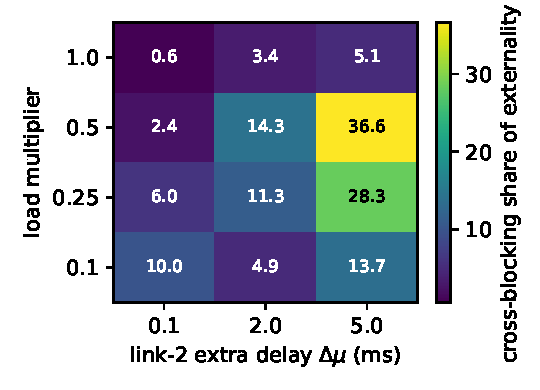
\includegraphics[width=0.5\linewidth]{fig_share.pdf}
\caption{Cross-blocking's share of the externality (\%) vs.\ load and asymmetry (\tagE{}).}
\end{figure}
Queueing/service delay accounts for \SBBNetMin{}--\SBBNetMax{} of the externality across cells, self-reordering for at most \SBBSelfAbs{} in absolute value, and cross-blocking for \SBBCrossMin{} (load \SBBMinCrossLoad{}, smallest asymmetry) up to \SBBCrossMax{} (load \SBBMaxCrossLoad{}, \SBBMaxCrossAsym{}~ms asymmetry), median \SBBCrossMed{}, below 15\% in \SBBCrossBelowFifteen{} cells. The share grows with link asymmetry and is largest at moderate load, as expected when reordering is frequent but queues are short. This also explains the V3 failure: at 25\% load with 2~ms asymmetry the share was well below the required 0.75. The quantities are sample means of per-packet delays over delivered packets (censoring is negligible at these horizons).

\section{Simulator and evaluation audit (Study 1)}\label{sec:audit}
Study 1 (hashes and commits in the Reproducibility section) preregistered six hypotheses about implicit invariants, with exact oracles and controls, on seeds 7000--7099.
\begin{table}[h]
\centering\small
\begin{tabular}{p{0.06\linewidth}p{0.52\linewidth}p{0.3\linewidth}}
\toprule
 & Primary measure & Outcome \\
\midrule
H1 & shared-stream arrival mismatches \OneMismatchShared{}; $\Delta\rho=\DeltaRhoTwo$ \DeltaRhoTwoCI{} & \HOneVerdictTwo{} \\
H2 & undelivered fraction \UndelFracFIFO{} (threshold \UndelThreshold) & \HTwoVerdict{} \\
H3 & paired-CI width ratio keyed/shared \WidthRatioTwo{} & \HThreeVerdictTwo{} \\
H4 & $|\Delta S_1|/S_1=\HFourRatioFIFO$ \HFourRatioFIFOCI{}; trace control \HFourTrace{} & violation \HFourVerdict{} \\
H5 & loss draws/attempt $\neq1$ in \OFiveRate{}; burst length \BurstShipped{} vs.\ \BurstSingle{} & \HFiveVerdict{} \\
H6 & violating seeds FIFO \HSixFIFO{}, FullSASP \HSixFullSASP{}, MeanOnly \HSixMeanOnly{}; leak control \HSixLeakyGlobal{} & \HSixVerdict{} \\
\bottomrule
\end{tabular}
\caption{Study 1 preregistered outcomes (\tagC{}).}
\end{table}
The shared random stream did not desynchronise arrivals; keyed noise did not tighten paired intervals (width ratio \WidthRatioTwo{}); survivor bias was immaterial. Three consequences matter for this paper. First, \textbf{H4}: self-blocking is invariant on a fixed trace but changed by \HFourRatioFIFO{} (about \HFourUnits{}~$\mu$s) when the competitor was removed from the system, the observation that motivated Study 2. Second, \textbf{H5}: every attempt drew two loss variables (\OFiveRate{}), shortening burst length by \BurstRelAbs{}; in an exploratory run absolute weighted blocking under bursts changed from \XTwoMShipFIFO{} to \XTwoMSingleFIFO{} while the FIFO-to-FullSASP reduction stayed near \XTwoRedShip{} (shipped) vs.\ \XTwoRedSingle{}. Third, \textbf{effect sizes}: the scheduler's gain in $M$ from 1000 fresh seeds is \XFourDShared{} (\XFourCIShared{}) against \OldD{} (\OldDCI{}) from the earlier 30-seed campaign, \OldRatio{}$\times$ larger but with overlapping intervals (\tagE{}, \tagP{}). Pairing between arms weakens with link asymmetry under both shared and keyed streams (Figure~\ref{fig:pair}, \tagE{}) and varies from \XFiveRhoMin{} to \XFiveRhoMax{} across pre-existing ns-3 cells while offered traffic was identical in \XFiveIdentical{} of \XFiveTriples{} triples, so weak pairing reflects scheduler-induced divergence, not random-number design. The causality check passed for all real schedulers but, at release level, could not see a one-millisecond look-ahead (\HSixLeakyLocal{}); a decision-level comparison caught it in \XThreeLeakyLocal{} (\tagE{}).
\begin{figure}[h]
\centering
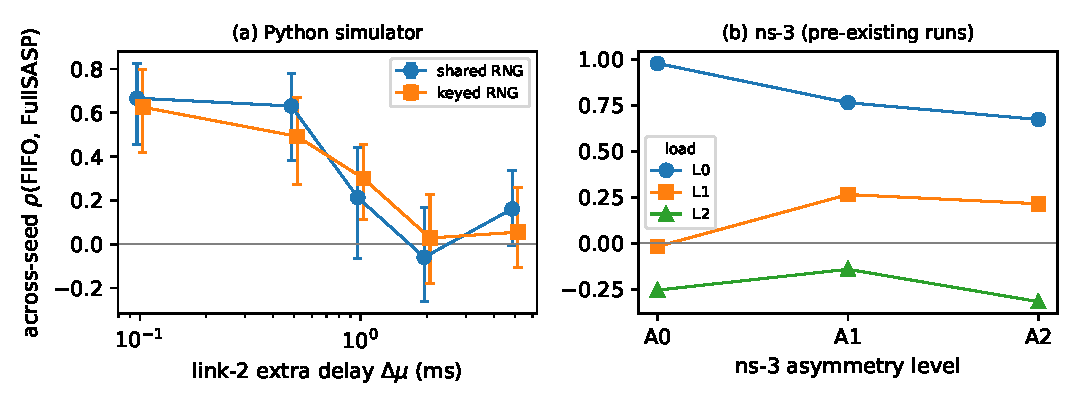
\includegraphics[width=0.9\linewidth]{fig_pairing.pdf}
\caption{Across-seed correlation between FIFO and FullSASP (\tagE{}; panel b: \tagP{}).}\label{fig:pair}
\end{figure}

\section{Claim-to-evidence table}
Tags: \tagC{} preregistered confirmatory; \tagE{} exploratory; \tagP{} analysis of pre-existing data; \tagA{} analytic.
\begin{table}[h]
\centering\footnotesize
\begin{tabular}{p{0.34\linewidth}p{0.3\linewidth}p{0.09\linewidth}p{0.17\linewidth}}
\toprule
Claim & Evidence & Tag & Result file \\
\midrule
Externality splits exactly into queueing, self, cross parts & identity gap \SBBIdentity{}; solo control \SBBSolo & \tagA/\tagE & exploratory\_study2b \\
Shapley blame is efficient & gap \SBVone & \tagA/\tagC & analysis\_study2 \\
Trace cross-blocking explains little at heavy load & \SBrFour{} \SBrFourCI & \tagC (V3 failed) & analysis\_study2 \\
Cross-blocking share depends on load and asymmetry & \SBBCrossMin{}--\SBBCrossMax & \tagE & exploratory\_study2b \\
Trace blame misranks flows & $\tau=\SBtauFour$ \SBtauFourCI & \tagC (V3 failed) & analysis\_study2 \\
Misranking persists under unequal flows (SASP) & $\tau=\SBSaspTau$ & \tagE & analysis\_study2 \\
Externalities are non-additive & $R=\SBRFour$ \SBRFourCI & \tagC & analysis\_study2 \\
Self-blocking invariant only on a trace & \HFourRatioFIFO{}; control \HFourTrace & \tagC & analysis \\
Two loss draws per attempt & \OFiveRate{} & \tagC & analysis \\
Double draw changes absolute $M$ & \XTwoMShipFIFO{} vs.\ \XTwoMSingleFIFO & \tagE & exploratory \\
Shared stream kept arrivals identical & \OneMismatchShared{} & \tagC & analysis \\
Gain estimate shrinks with more seeds & \OldD{} vs.\ \XFourDShared & \tagE/\tagP & exploratory \\
Pairing weakens with asymmetry/load & \XOneRhoLow{}$\to$\XOneRhoHigh;\ ns-3 \XFiveRhoMin{}--\XFiveRhoMax & \tagE/\tagP & exploratory \\
When trace equals interventional (pinned disjoint links) & Proposition~\ref{prop:cond} & \tagA{} (untested) & --- \\
\bottomrule
\end{tabular}
\caption{Every number resolves to a stored result file through \texttt{make\_numbers.py}.}
\end{table}

\section{Discussion}
The practical message is about what to measure. A reordering-delay figure that looks small does not mean the flows are independent: here the dominant cross-flow harm was queueing, which a trace-based blocking metric cannot see, and blame assigned from traces did not identify the flows whose removal helps most. For scheduler design the externality suggests an objective (charge each dispatch its marginal harm to others) that we have \emph{not} tested; we mention it as future work only. Pinning flows to disjoint links makes the two notions coincide (Proposition~\ref{prop:cond}) at the cost of load balancing, a trade-off worth quantifying.

\section{Limitations}
\begin{itemize}
  \item \textbf{The validity control failed.} V3 was \SBVthreeStatus{}; the confirmatory verdicts H7--H9 are therefore not independently validated, and the replacement evidence (identity, sweep) is exploratory.
  \item One simulator, two links, 300~ms runs, FIFO as the primary arm. Shares are regime-dependent (\SBBCrossMin{}--\SBBCrossMax{}); no general magnitude is claimed.
  \item Under FIFO the flows are nearly exchangeable, so the ranking test (H8) has little signal; the unequal-flow evidence (SASP) is exploratory.
  \item The Shapley value is one attribution; with strongly convex externalities ($R=\SBRFour$) other allocations (for example marginal-cost pricing) answer different questions. We did not compare allocations.
  \item Means are over delivered packets in Study 2b; Study 2 uses right-censored means. Censoring was negligible at these horizons but was not varied.
  \item The audit's pilot seeds 1--40 were examined before an amendment (disclosed in the preregistration); confirmatory seeds were untouched. Study 2 and 2b used fresh seeds.
  \item The ns-3 material re-analyses runs made before this work; no new ns-3 experiments were run.
  \item The literature search was limited. Unverifiable inherited references were excluded.
  \item $p$-values (Study 1) use a sign-flip test instead of a $t$-test; no human annotation, model judge or hardware measurement was used.
\end{itemize}

\section{Conclusion}
Separating what a trace says from what an intervention changes shows that, in this simulator, cross-flow reordering delay is mostly not what a trace-based cross-blocking metric reports, and that blame inferred from traces does not rank the offending flows like an exact counterfactual attribution does. The contribution is a measurement concept with an exact identity and falsifiable checks, one failed control reported as such, and an audit that makes the supporting machinery trustworthy. Whether externality-aware scheduling pays off remains open.

\section*{Reproducibility}\label{sec:repro}
All materials are in \texttt{validation/pairing/}. Study 1: preregistration \texttt{4f4b8f0} (SHA-256 \texttt{abf0c16a\dots}), Amendment~1 \texttt{d7448bb}, Amendment~2 and harness \texttt{25d2ce1}, results and exploratory plan \texttt{49437e6}. Study 2: preregistration \texttt{87e5f67} (SHA-256 \texttt{73c53be0\dots}); results, V3 failure and Study 2b plan \texttt{30408d9}. Raw-file hashes: \texttt{results/RAW\_AND\_ANALYSIS.sha256}, \texttt{results/STUDY2\_RAW.sha256}. Rebuild with \texttt{run\_study.py}, \texttt{analyze.py}, \texttt{run\_exploratory.py}, \texttt{run\_study2.py}, \texttt{analyze\_study2.py}, \texttt{run\_study2b.py}, then \texttt{paper/make\_numbers.py} and \texttt{paper/make\_fig.py}. Decisions are logged in \texttt{decisions.md}.

\bibliographystyle{plain}
\bibliography{refs}
\end{document}
